\documentclass[a4paper,11pt]{article}

\usepackage[T1]{fontenc}
\usepackage[utf8]{inputenc}
\usepackage{lmodern}
\usepackage{microtype}
\renewcommand{\familydefault}{\sfdefault}
\usepackage[english]{babel}
\usepackage[left=1.5cm,right=1.5cm,top=1.8cm,bottom=2.0cm]{geometry}
\usepackage[parfill]{parskip}
\usepackage[dvipsnames,table]{xcolor}
\usepackage{amsmath,amssymb,amsfonts}
\usepackage{graphicx}
\usepackage{float}
\usepackage[skip=1.5ex]{caption}
\captionsetup{font=small,labelsep=period}
\usepackage{array,booktabs,tabularx,multirow}
\renewcommand{\arraystretch}{1.25}
\usepackage[inline]{enumitem}
\usepackage{tikz}
\usetikzlibrary{arrows.meta,decorations.pathreplacing,positioning,calc,shapes.geometric,decorations.pathmorphing,fit,backgrounds}
\usepackage[most]{tcolorbox}
\usepackage{titlesec}
\usepackage{fancyhdr}
\usepackage[pdfusetitle,colorlinks=true,linktoc=all,allcolors=Blue]{hyperref}
\usepackage{bookmark}
\usepackage{doi}

%%%%%%%%%%%%%%%%%%%%
% Colours           %
%%%%%%%%%%%%%%%%%%%%
\definecolor{mysectioncolor}{HTML}{3F51B5}
\definecolor{mysubsectioncolor}{HTML}{355E3B}
\definecolor{darkerred}{RGB}{80,0,0}
\definecolor{aimblue}{HTML}{004c8c}
\definecolor{aimbg}{HTML}{f4f8fb}
\definecolor{iceblue}{RGB}{210,230,250}
\definecolor{DarkRed}{RGB}{140,0,0}

% Equipment colour code (= what the item is used for)
\definecolor{cCtrl}{HTML}{1F5FBF} % operate / inputs / outputs
\definecolor{cSamp}{HTML}{2E8B57} % sample characterisation (phi, density, volume, mass)
\definecolor{cEnv}{HTML}{D96F00}  % environment (T, salinity)
\definecolor{cImg}{HTML}{8A3FB5}  % imaging / visual record
\definecolor{cMech}{HTML}{4D4D4D} % mechanics (rheometer + deployment)

%%%%%%%%%%%%%%%%%%%%
% Sections / header %
%%%%%%%%%%%%%%%%%%%%
\titleformat{\section}{\color{mysectioncolor}\normalfont\Large\bfseries}{\thesection}{1em}{}
\titleformat{\subsection}{\color{darkerred}\normalfont\large\bfseries}{\thesubsection}{1em}{}
\titleformat{\subsubsection}{\color{mysubsectioncolor}\normalfont\normalsize\bfseries}{\thesubsubsection}{1em}{}
\setcounter{secnumdepth}{3}
\setcounter{tocdepth}{2}
\pagestyle{fancy}\fancyhead{}\fancyfoot{}\fancyfoot[C]{\thepage}\renewcommand{\headrulewidth}{0pt}

%%%%%%%%%%%%%%%%%%%%
% Helpers           %
%%%%%%%%%%%%%%%%%%%%
\newcolumntype{Y}{>{\raggedright\arraybackslash}X}
\newcommand{\todo}[1]{\textcolor{red}{[#1]}}
\newcommand{\fillme}{\textcolor{red}{[\hspace{1.2em}]}}   % blank to be filled later
\newcommand{\code}[1]{\texttt{#1}}
\newcommand{\safeimg}[2][]{\IfFileExists{#2}{\includegraphics[#1]{#2}}{\fbox{\scriptsize missing: \detokenize{#2}}}}
\newcommand{\logo}[3][0pt]{\raisebox{-0.5\height}{\raisebox{#1}{\safeimg[height=#2]{#3}}}}

% Equipment badges: \badge{colour}{label}
\newcommand{\badge}[2]{{\setlength{\fboxsep}{1.8pt}\colorbox{#1}{\textcolor{white}{\scriptsize\textbf{#2}}}}}
\newcommand{\eqChip}{\badge{cMech}{CHIP}}  % Chipiron
\newcommand{\eqFlt}{\badge{cMech}{FLT}}    % floating pieces
\newcommand{\eqPC}{\badge{cCtrl}{PC}}      % laptop
\newcommand{\eqArd}{\badge{cCtrl}{ARD}}    % Arduino / current acquisition
\newcommand{\eqEsc}{\badge{cCtrl}{ESC}}    % ESCON Studio
\newcommand{\eqPy}{\badge{cCtrl}{PY}}      % Python acquisition / processing
\newcommand{\eqGrad}{\badge{cSamp}{GRAD}}  % graduated volume container
\newcommand{\eqBal}{\badge{cSamp}{BAL}}    % balance
\newcommand{\eqSmp}{\badge{cSamp}{SMP}}    % frazil sampler
\newcommand{\eqFil}{\badge{cSamp}{FIL}}    % filter / mesh
\newcommand{\eqFzm}{\badge{cSamp}{FZM}}    % frazilometer
\newcommand{\eqCont}{\badge{cSamp}{CONT}}  % sample container
\newcommand{\eqThm}{\badge{cEnv}{THM}}     % thermometer
\newcommand{\eqCnd}{\badge{cEnv}{CND}}     % conductimeter / salinity
\newcommand{\eqCam}{\badge{cImg}{CAM}}     % phone / camera
\newcommand{\eqMic}{\badge{cImg}{MIC}}     % microscope / macro camera

\newcommand{\stepno}[1]{\textbf{#1}}

% Flowchart styles
\tikzset{
  fstep/.style={draw=aimblue,fill=aimbg,rounded corners=3pt,align=center,text width=3.2cm,minimum height=1.25cm,font=\footnotesize,inner sep=3pt},
  fdec/.style={fstep,draw=DarkRed,fill=red!6},
  fphase/.style={fstep,fill=aimblue,text=white,draw=aimblue},
  fok/.style={fstep,draw=mysubsectioncolor,fill=green!8},
  arr/.style={-{Stealth[length=2.2mm]},thick,aimblue},
  lab/.style={font=\scriptsize\itshape,fill=white,inner sep=1pt}
}

\begin{document}

%%%%%%%%%%%%%%%%%%%%
% TITLE PAGE        %
%%%%%%%%%%%%%%%%%%%%
\pagenumbering{roman}
\thispagestyle{empty}
\vspace*{-2.2cm}
\noindent\makebox[\textwidth]{%
  \logo{1cm}{figures/AS.png}\hfil
  \logo{2cm}{figures/logopmmh1.png}\hfil
  \logo{3.6cm}{figures/ISTERRElogo.png}\hfil
  \logo{1.6cm}{figures/logo-blue.png}\hfil
  \logo{0.8cm}{figures/logoSPI.png}\hfil
  \logo{1cm}{figures/logoUQAR.jpg}}
\vspace{4cm}
\begin{center}
  {\Huge\bfseries CASCADES26 Expedition}\\[0.5em]
  {\Large\bfseries CGGS Amundsen}\\[2em]
  {\huge\color{mysectioncolor}\bfseries FMeasurement scenarios for Chipiron}\\[3em]
  {\Large\bfseries Matilde Bureau}\\[1em]
  {\large \href{mailto:matilde.bureau@espci.fr}{matilde.bureau@espci.fr}}\\[2em]
  {\large \today}
\end{center}
\vfill\newpage

\thispagestyle{empty}
\tableofcontents
\newpage
\pagenumbering{arabic}\setcounter{page}{1}

%=========================================================
\section{Conventions \& definitions of key quantities}\label{sec:conv}
%=========================================================

\subsection{System sketch and quantities: frazil rheology}

\begin{figure}[H]
\centering
\resizebox{\linewidth}{!}{%
\begin{tikzpicture}[>=Stealth]
% air / water
\fill[blue!8] (0,-3.2) rectangle (11.6,0);
\draw[blue!50] (0,0) -- (11.6,0);
% floes
\fill[white,draw=blue!60,thick] (0,-0.5) rectangle (2.8,0.15);
\fill[white,draw=blue!60,thick] (9.2,-0.5) rectangle (11.6,0.15);
\node[font=\scriptsize,blue!60!black] at (1.4,-0.17) {floe};
\node[font=\scriptsize,blue!60!black] at (10.4,-0.17) {floe};
% frazil layer
\fill[iceblue!60] (2.8,0) rectangle (9.2,-0.95);
\foreach \i in {1,...,80}{
  \pgfmathsetmacro{\cx}{2.95+mod(\i*53,61)/10}
  \pgfmathsetmacro{\cy}{-0.1-mod(\i*29,76)/100}
  \pgfmathsetmacro{\ca}{mod(\i*67,180)}
  \draw[rotate around={\ca:(\cx,\cy)},fill=white,draw=blue!60] (\cx,\cy) ellipse (0.14 and 0.04);
}
% thickness h0
\draw[<->,thick,DarkRed] (3.0,0) -- (3.0,-0.95) node[bottom,left=1pt,fill=none,inner sep=1pt,font=\small] {$h_0$};
% water label
\node[font=\small,blue!60!black] at (6,-2.4) {water};
% vane + motor
\draw[very thick,cMech] (6,2.0) -- (6,-1.15);
\draw[very thick,cMech] (5.55,-0.25) -- (6.45,-0.25);
\draw[very thick,cMech] (5.55,-1.1) -- (6.45,-1.1);
\draw[very thick,cMech] (5.55,-0.25) -- (5.55,-1.1);
\draw[very thick,cMech] (6.45,-0.25) -- (6.45,-1.1);
\node[draw=cMech,fill=cMech!15,minimum width=1.4cm,minimum height=0.6cm,font=\small] at (6,2.3) {motor};
% immersion depth
\draw[<->,cMech] (6.9,0) -- (6.9,-1.1) node[top,right=1pt,font=\small] {$d$};
% omega
\draw[-{Stealth},thick,cCtrl] (5.2,1.35) to[bend left=50] (6.8,1.35);
\node[cCtrl,font=\small] at (6.3,1.4) {$\omega$};
% inputs / outputs
\node[cCtrl,font=\small,align=left,anchor=east] at (5.0,2.3) {input: $U$\\output: $I\to\tau$};
% phi definition

\node[font=\small,align=center,fill=white] at (6,-1.75) {Frazil: $\phi = V_i/V_g, ~\nu_{eff}, ~ T_g, ~ S_g, ~ \rho_g$ };
% oscillation inset
\node[font=\small\bfseries] at (14.9,2.6) {oscillatory mode $ \tau = G\gamma, ~G = G' + iG''$};
\draw[->] (12.4,1.15) -- (17.6,1.15) node[right,font=\small]{$t$};
\draw[blue!70!black,thick,domain=0:6.28,samples=60,variable=\t] plot ({12.5+\t*0.75},{1.15+0.6*sin(\t r)});
\node[blue!70!black,font=\small] at (14.9,1.95) {$\gamma(t)=\gamma_0\sin(2\pi f t)$};
\draw[->] (12.4,-0.6) -- (17.6,-0.6) node[right,font=\small]{$t$};
\draw[red!70!black,thick,domain=0:6.28,samples=60,variable=\t] plot ({12.5+\t*0.75},{-0.6+0.6*sin(\t r+0.8)});
\node[red!70!black,font=\small] at (14.9,0.2) {$\tau(t)\tau_0\sin(2\pi f t + \delta)$};
\node[font=\small,align=left,anchor=north west] at (12.4,-1.4) {$G'\propto\cos\delta$: in-phase/elastic\\[2pt]
 $G''\propto\sin\delta$: quadrature/viscous\\[2pt]
 $\gamma_{\rm fl}$: fluidization transition};
\end{tikzpicture}}
\caption{Chipiron in a frazil layer between floes. Continuous mode: imposed $\omega$, measured $\tau$. Oscillatory mode: imposed $\gamma(t)$, measured $\tau(t)$.}
\label{fig:sketch}
\end{figure}

\begin{table}[H]
\centering
\begin{tabularx}{\textwidth}{@{}l Y Y@{}}
\toprule
\textbf{Symbol} & \textbf{Meaning} & \textbf{Obtained from} \\
\midrule
\multicolumn{3}{@{}l}{\textit{Imposed / measured by the rheometer}}\\
$U$ & motor input voltage & imposed (\eqPC\,\eqEsc) \\
$\omega$ & rotation speed (continuous mode) & imposed via $U$; check with calibration (\S\ref{sec:transit}) \\
$I,\ \tau$ & motor current, torque & measured (\eqArd), $\tau\propto I$ \\
$\gamma_0,\ f$ & forcing strain amplitude/frequency (oscillatory mode) & imposed via $U$ \\
$G',\ G''$ & storage / loss modulus (oscillatory mode) & from $\tau(t)$ vs.\ $\gamma(t)$ \\
$\delta$ & phase shift between $\gamma$ and $\tau$ & measured \\
$\gamma_{\rm fl}$ & fluidization & from $G'(\gamma_0),G''(\gamma_0)$ \\
$\nu_{\rm eff}$ & effective viscosity & from viscous response \\
$J$ & inertia number  & from $\tau(\omega)$ \\
\midrule
\multicolumn{3}{@{}l}{\textit{Frazil state}}\\
$\phi=V_i/V_g$ & solid fraction & \eqSmp\,\eqFil\,\eqGrad\,\eqBal; \cite{MausDeLaRosa2012} \\
$h_0$ & frazil layer thickness & field estimate \\
$V_g,\ m_g$ & sample volume, mass & \eqGrad, \eqBal \\
$T_g,\ S_g$ & sample temperature, salinity & \eqThm, \eqCnd \\
$d$ & vane immersion depth & geometry \\
\bottomrule
\end{tabularx}
\caption{Quantities used throughout for ocntinuous ad oscillatory rheology experiments. }
\end{table}

\subsection{Equipment symbols and colour code}
Colour = what the item is used for. The symbols are used everywhere in the rest of the document.

\begin{table}[H]
\centering
\begin{tabularx}{\textwidth}{@{}c l Y c c@{}}
\toprule
\textbf{Symbol} & \textbf{Item} & \textbf{Purpose} & \textbf{Field} & \textbf{Lab} \\
\midrule
\rowcolor{cCtrl!10}\multicolumn{5}{@{}l}{\textbf{Blue --- Inputs/outputs}}\\
\eqPC  & laptop & runs everything below & \checkmark & \checkmark \\
\eqArd & Arduino / current measurement & acquires $I$ and $U$ & \checkmark & \checkmark \\
\eqEsc & ESCON Studio & motor control / imposes $U$ & \checkmark & \checkmark \\
\eqPy  & Python scripts & acquisition and processing & \checkmark & \checkmark \\
\midrule
\rowcolor{cMech!10}\multicolumn{5}{@{}l}{\textbf{Grey --- mechanics}}\\
\eqChip & Chipiron (rheometer) & measures $\tau(\omega)$, $G',G''$ & \checkmark & \checkmark \\
\eqFlt & floating pieces & keeps Chipiron at the right depth $d$ & \checkmark & --- \\
\midrule
\rowcolor{cSamp!10}\multicolumn{5}{@{}l}{\textbf{Green --- sample characterization ($\phi$, density, volume, mass)}}\\
\eqSmp  & frazil sampler & get sample and possibly filter it & \checkmark & \checkmark \\
\eqFil  & filter / mesh & crystal--brine separation & \checkmark & \checkmark \\
\eqGrad & graduated volume container & $V_g$, $V_i$ & \checkmark & \checkmark \\
\eqBal  & balance & $m_g$ & \checkmark & \checkmark \\
\eqFzm  & frazilometers & local frazil thickness & \checkmark & --- \\
\eqCont & sample containers & for lab rheology and/or characterization & \checkmark & \checkmark \\
\midrule
\rowcolor{cEnv!10}\multicolumn{5}{@{}l}{\textbf{Orange --- environment}}\\
\eqThm & thermometer & $T$ (air, water, sample) & \checkmark & \checkmark \\
\eqCnd & conductimeter / salinity & $S$ (if available) & (\checkmark) & \checkmark \\
\midrule
\rowcolor{cImg!10}\multicolumn{5}{@{}l}{\textbf{Purple --- visual record}}\\
\eqCam & phone / camera & before / during / after pictures & \checkmark & \checkmark \\
\eqMic & optics/ camera & crystal size, aspect ratio & (optional) & (optional) \\
\bottomrule
\end{tabularx}
\caption{Equipment legend.}
\end{table}

\subsection{Scripts}
\begin{table}[H]
\centering
\begin{tabularx}{\textwidth}{@{}l l Y@{}}
\toprule
\textbf{Purpose} & \textbf{Script} & \textbf{Command / parameters} \\
\midrule
Plan $\omega$ ramp (log / lin) & \code{Ramp\_planning\_Chipiron.py} & \fillme \\
Plan $\gamma_0$ sweep (log / lin) & \code{Oscill\_sweep\_planning\_Chipiron.py} & \fillme \\
Execute a run & \code{run.py} & \fillme \\
Analysis / quick check & \fillme & \fillme \\
Sample characterization & \fillme & \fillme \\
\bottomrule
\end{tabularx}
\caption{Scripts (\eqPy). Empty = not decided / not known.}
\label{tab:scripts}
\end{table}

%=========================================================
\section{CASCADES pipeline}\label{sec:master}
%=========================================================
\begin{figure}[H]
\centering
\begin{tikzpicture}[node distance=1.0cm]
\node[fphase] (T) {\textbf{TRANSIT}\\calibrate, find input ranges\\(\S\ref{sec:transit})};
\node[fdec,right=of T] (W) {Where am I?};
\node[fstep,above right=0.2cm and 1.0cm of W] (F) {\textbf{FIELD}\\pipeline (\S\ref{sec:field})};
\node[fstep,below right=0.2cm and 1.0cm of W] (L) {\textbf{LAB}\\pipeline (\S\ref{sec:lab})};
\node[fok,right=4.3cm of W] (R) {\textbf{Repeatability first}\\same state, same protocol, $N$ repeats};
\draw[arr] (T) -- (W);
\draw[arr] (W.east) -- (F.west);
\draw[arr] (W.east) -- (L.west);
\draw[arr] (F.east) -- (R.north west);
\draw[arr] (L.east) -- (R.south west);
\end{tikzpicture}
\caption{Overall steps. Note: focus on repeatabilit yto make sure we have robust data. Parameter variations only come afterwards. (\S\ref{sec:deferred}).}
\end{figure}



%=========================================================
\section{Transit period}\label{sec:transit}
%=========================================================
Frazil can already be sampled and the setup tested during transit. Goal: calibrate quantities, identify usable ranges, set parameters for all tests.

\begin{figure}[H]
\centering
\begin{tikzpicture}[node distance=0.75cm]

\node[fstep] (a) {\stepno{1} Test chain\\\eqPC\,\eqArd\,\eqEsc\,\eqChip\\zero / check signal};

\node[fstep,right=of a] (b) {\stepno{2} Calibrate\\$U\to\omega$};

\node[fstep,right=of b] (c) {\stepno{3} Calibrate\\$U\to\gamma$};

\node[fstep,below=0.9cm of c] (d) {\stepno{4} Find usable ranges\\$\omega$ and $\gamma_0$ (in $U$)};

\node[fstep,left=of d] (e) {\stepno{5} Repeatability test:\\identical runs};

\node[fstep,left=of e] (f) {\stepno{6} Hysteresis\\desc.\ vs asc. + pre-shear tests: decide protocol.};

\node[fstep,below=0.9cm of e] (g) {\stepno{7} Decide typical exp.\ params\\fill default params. tables in  \S\ref{sec:protocols} and tab.\ref{tab:transit}};

\node[fstep,below=0.9cm of g] (h) {\stepno{8} Practice sample characterization \cite{MausDeLaRosa2012} to get $\phi$};

\draw[arr] (a)--(b);
\draw[arr] (b)--(c);
\draw[arr] (c)--(d);
\draw[arr] (d)--(e);
\draw[arr] (e)--(f);
\draw[arr] (f.south)--++(0,-0.5)|-(g.west);
\draw[arr] (g)--(h);

\end{tikzpicture}
\caption{Transit pipeline.}
\end{figure}


\begin{table}[H]
\label{tab:transit}
\centering
\begin{tabularx}{\textwidth}{@{}l Y Y Y Y@{}}
\toprule
\textbf{Quantity to find} & \textbf{Range} & \textbf{N pts} & \textbf{Time / pt} & \textbf{Default} \\
\midrule
$\omega$ (ramp) & \fillme & \fillme & \fillme & \fillme \\
$\gamma_0$ (oscill.) & \fillme & \fillme & \fillme & \fillme \\
$f$ (oscill.) & \fillme & \fillme & \fillme & \fillme \\
\bottomrule
\end{tabularx}
\caption{Experimental ranges to test. }
\end{table}

\newpage
%=========================================================
\section{Field case}\label{sec:field}
%=========================================================
\subsection{Pipeline}
\begin{figure}[H]
\centering
\resizebox{\textwidth}{!}{%
\begin{tikzpicture}[node distance=0.75cm]

\node[fstep] (n1) {\stepno{1} PLAN\\1\,h meeting: which measurements today?};

\node[fstep,right=of n1] (n2) {\stepno{2} SETUP (10 min)\\
\eqChip\,\eqPC\,\eqArd\,\eqEsc\\
check signals sent/received; \eqFlt};

\node[fstep,right=of n2] (n3) {\stepno{3} DEPLOY (40 min)\\
\eqChip\ in frazil at depth $d$};

\node[fstep,right=0.55cm of n3] (n4) {\stepno{4} CHARACTERIZE\\
$\phi,\ h_0,\ T,\ S$\\
\eqSmp\,\eqFzm\,\eqThm\,\eqCnd\,\eqCam};

\node[fdec,below=1.0cm of n4] (n5)
{\stepno{5} Which measurement?};

\node[fstep,left=1.3cm of n5,yshift=0.7cm] (n6a)
{\stepno{6a} Continuous\\$\omega$-ramp (\S\ref{sec:ramp})};

\node[fstep,left=1.3cm of n5,yshift=-0.7cm] (n6b)
{\stepno{6b} Oscillatory\\$\gamma_0$ sweep (\S\ref{sec:osc})};

\node[fstep,left=1.3cm of n6a,yshift=-0.7cm] (n7)
{\stepno{7} REPEAT\\same location and protocol};

\node[fstep,left=of n7] (n8)
{\stepno{8} SAVE\\raw data, metadata, pictures of test};

% Optional step
\node[fstep,below=0.9cm of n8,xshift=1.5cm,
      text width=9.5cm,align=center] (n9)
{\stepno{9} OPTIONAL\quad
(i) Vary location and/or sample depth and repeat protocol
\quad (ii) Same location/depth: vary $f$, $\gamma_0$ range (oscill.)
or $\omega$ range (continuous)};

% Final step, to the right of Step 9
\node[fstep,right=0.6cm of n9,text width=3.2cm,align=center] (n10)
{\stepno{10} BACK ON BOARD\\30 min};

\draw[arr] (n1)--(n2); 
\draw[arr] (n2)--(n3); 
\draw[arr] (n3)--(n4);
\draw[arr] (n4)--(n5);

\draw[arr] (n5.west)--(n6a.east);
\draw[arr] (n5.west)--(n6b.east);

\draw[arr] (n6a.west)--(n7.east); 
\draw[arr] (n6b.west)--(n7.east);

\draw[arr] (n7)--(n8);
\draw[arr] (n8)--(n9);
\draw[arr] (n9)--(n10);

\end{tikzpicture}%
}
\caption{Field pipeline.}
\end{figure}
% \subsection{Time budget and roles}
% \begin{table}[H]
% \centering
% \begin{tabularx}{\textwidth}{@{}l c Y@{}}
% \toprule
% \textbf{Step} & \textbf{Duration} & \textbf{Note} \\
% \midrule
% Plan & 1\,h & meeting \\
% Setup & 10\,min & \eqChip\ inspect / connect; \eqPC\,\eqArd\,\eqEsc; zero / check; \eqFlt; agree position \\
% Deployment (in / out) & 40\,min each \todo{?} & \\
% Active measurement (ramp) & $\le$ 50\,min & worst case: 100 pts over 7 decades, 30\,s / pt \\
% Sample characterisation (oscillatory) & 20\,min or more & $\phi$ (\eqSmp\ or density / conductivity), $h_0$; longer with filtering protocol \\
% Active measurement (oscillatory) & \fillme & check Foulques' notes: duration of one sweep at given $f$ \\
% Repeats & $\times$3--4 \todo{?} & same location, if frazil state stays comparable \\
% \textbf{Total} & $\approx$ 2\,h10 per sweep & 4--6\,h if several measurements \todo{?} \\
% \bottomrule
% \end{tabularx}
% \caption{Field time budget.}
% \end{table}

\begin{table}[H]
\centering
\begin{tabularx}{\textwidth}{@{}l Y@{}}
\toprule
\textbf{Role (3 people)} & \textbf{Actions} \\
\midrule
Deck handler & sends inputs, runs \eqPC\,\eqEsc, records run ID + metadata, checks live $I/\tau$ (and waveform quality in oscillatory mode) \\
Operators 1 \& 2 & position \eqChip\ in the frazil layer, keep geometry / depth $d$, \eqCam\ local frazil, record ice type, $h_0$, location, wave state, wind, obtain $\phi$ \\
\bottomrule
\end{tabularx}
\caption{Field roles. }
\end{table}

\subsection{Outputs}
\begin{enumerate}[label=\textbf{\arabic*.},nosep]
  \item \textbf{Context}: date/time, GPS, floe / water configuration, waves, wind, $T_{\rm air}$, $T_{\rm water}$, $S$
  \item \textbf{Frazil}: ice type, $\phi$, $h_0$, $T$, crystal size / shape
  \item \textbf{Geometry}: vane type, $d$, position vs.\ floe edge, sample depth
   \item \textbf{Inputs}: all rows of the protocol table (\S\ref{sec:protocols})
  \item \textbf{Raw data}: full $I/\tau$ and $U$ time series (\eqPC\,\eqArd)
  \item \textbf{Pictures / video}: before, during, after (\eqCam)
  \item \textbf{Sample history:} previous tests if any, pre-shear if any, visible qualitative structural change 
  \item \textbf{Side sample} from same place and depth: $\phi$, $T$, $S$, $m$, $V$, crystal size (\eqSmp\,\eqFil\,\eqGrad\,\eqBal)
\end{enumerate}

\begin{table}[H]
\centering
\begin{tabularx}{\textwidth}{@{}c Y@{}}
\toprule
\textbf{Priority order} &  \\
\midrule
1 & one good descending $\omega$ ramp + full raw series + local $\phi,h_0$ + context \\
2 & repeat same ramp (repeatability / history) \\
3 & one oscillatory amplitude sweep  \\
4 & repeat same oscillatory sweep  \\
5 & Other location/sampling depth, record changes in $\phi$, $h_0$ \\
6 & more $f$ values (oscillatory) \\
\bottomrule
\end{tabularx}
\end{table}

\newpage
%=========================================================
\section{Lab case}\label{sec:lab}
%=========================================================
\subsection{Pipeline}
\begin{figure}[H]
\centering
\resizebox{\textwidth}{!}{%
\begin{tikzpicture}[node distance=0.75cm]

\node[fstep] (n1) {\stepno{1} PLAN (1h)\\ meeting: precise measurement plan};

\node[fstep,right=of n1] (n2) {\stepno{2} SAMPLE frazil (30 min)\\
\eqSmp\,\eqCont\\record $T_g$ (\eqThm)};

\node[fstep,right=of n2] (n3) {\stepno{3} SETUP ($\approx$ 20 min)\\
install \eqChip\ in \eqCont;\ \eqPC\,\eqArd\,\eqEsc};

\node[fstep,right=of n3] (n4) {\stepno{4} CHARACTERIZE ($\approx$ 30 min?)\\
$V_g,m_g,T_g,S_g,\phi$\\
\eqGrad\,\eqBal\,\eqFil\\
\eqThm\,\eqCnd\,\eqCam};

\node[fdec,below=1.0cm of n4] (n5)
{\stepno{5} Which measurement?};

\node[fstep,left=1.3cm of n5,yshift=0.7cm] (n6a)
{\stepno{6a} Continuous\\$\omega$-ramp (\S\ref{sec:ramp})};

\node[fstep,left=1.3cm of n5,yshift=-0.7cm] (n6b)
{\stepno{6b} Oscillatory\\$\gamma_0$ sweep (\S\ref{sec:osc})};

\node[fstep,left=1.3cm of n6a,yshift=-0.7cm] (n7)
{\stepno{7} REPEAT\\2--3 sweeps, same prepared sample};

\node[fstep,left=of n7] (n8)
{\stepno{8} SAVE\\raw data, metadata};

% Optional step
\node[fstep,below=0.9cm of n8,xshift=1.5cm,
      text width=9.5cm,align=center] (n9)
{\stepno{9} OPTIONAL\quad
(i) Vary one parameter ($\phi, ~ h_0, ~T_g$) and repeat measurements
\quad (ii) Vary $f$, $\gamma_0$ range (oscill.)
or $\omega$ range (continuous) \quad (iii) Follow rheology change across freezing if possible};

\draw[arr] (n1)--(n2); 
\draw[arr] (n2)--(n3); 
\draw[arr] (n3)--(n4);

\draw[arr] (n4)--(n5);

\draw[arr] (n5.west)--(n6a.east); 
\draw[arr] (n5.west)--(n6b.east);

\draw[arr] (n6a.west)--(n7.east); 
\draw[arr] (n6b.west)--(n7.east);

\draw[arr] (n7)--(n8);
\draw[arr] (n8)--(n9);

\end{tikzpicture}%
}
\caption{Lab pipeline.}
\end{figure}

\subsection{Roles}
% \begin{table}[H]
% \centering
% \begin{tabularx}{\textwidth}{@{}l c Y@{}}
% \toprule
% \textbf{Step} & \textbf{Duration} & \textbf{Note} \\
% \midrule
% Plan & 1\,h & meeting \\
% Setup & $\approx$1\,h \todo{?} & sample frazil, record $T_g$, install \eqChip \\
% Characterisation & $\approx$40\,min (ramp case) / 20--30\,min per sample (oscillatory case) & minimum set: $V_g,m_g,T_g,S_g$, visual crystal size; longer if crystal / brine separation \cite{MausDeLaRosa2012} \\
% Active measurement (ramp) & \fillme & check in Foulques' data \\
% Active measurement (oscillatory) & \fillme & amplitude sweep and frequency sweep: check Foulques' notes \\
% Replicates & 2--3 \todo{?} & same prepared sample (repeatability / history); for amplitude sweeps: how many? \\
% \textbf{Total} & \fillme & \\
% \bottomrule
% \end{tabularx}
% \caption{Lab time budget.}
% \end{table}

\begin{table}[H]
\centering
\begin{tabularx}{\textwidth}{@{}l Y@{}}
\toprule
\textbf{Role (2 people)} & \textbf{Actions} \\
\midrule
Operator 1 & controls \eqChip\ / acquisition (\eqPC\,\eqArd\,\eqEsc), checks live outputs, records run IDs, exact protocol, sample history \\
Operator 2 & prepares and characterizes the sample (\eqGrad\,\eqBal\,\eqFil\,\eqThm\,\eqCnd), follows temperature / ice state / structural change \\
\bottomrule
\end{tabularx}
\end{table}

\subsection{Outputs}
\begin{enumerate}[label=\textbf{\arabic*.},nosep]
  \item \textbf{Context}: date/time, GPS, sampling context (depth, waves, wind), $T_{\rm room}$, $T_{\rm sample}$, $S$
  \item \textbf{Frazil}: ice type, $\phi$, $h_0$, $T$, crystal size / shape, $V_g, ~ T_g, ~ S_g, ~\rho_g$
  \item \textbf{Geometry}: vane / rotor geometry, $d$, container dimensions, distance to walls / bottom, corrections / calibration used
   \item \textbf{Inputs}: all rows of the protocol table (\S\ref{sec:protocols})
  \item \textbf{Raw data}: full $I/\tau$ and $U$ time series (\eqPC\,\eqArd)
  \item \textbf{Pictures / video}: before, during, after (\eqCam)
  \item \textbf{Sample history:} previous tests if any, pre-shear if any, visible qualitative structural change 

\end{enumerate}

\begin{table}[H]
\centering
\begin{tabularx}{\textwidth}{@{}c Y@{}}
\toprule
\textbf{Priority order} &  \\
\midrule
1 & one descending $\omega$ ramp + full raw series +  $\phi,h_0$ + sample context \\
2 & repeat the ramp (repeatability / history) \\
3 & one oscillatory amplitude sweep  \\
4 & repeat oscillatory exp. \\
5 & vary available parameters ($\phi, ~ h_0, ~ T_g$, time after sampling) \\
6 & vary sweep amplitudes/frequencies (oscill.) \\
7 & perform frequency (not amplitude) sweep for oscill. measurements ? \\
8 & follow rheology across freezing if controlled conditions allow it  \\


\bottomrule
\end{tabularx}
\end{table}



\newpage
%=========================================================
\section{Measurement protocols (field and lab)}\label{sec:protocols}
%=========================================================
 ``Range / N pts / time per pt'' refer to the swept quantity; script commands are in Table~\ref{tab:scripts}.

\subsection{A --- Continuous: descending $\omega$ ramp}\label{sec:ramp}
\begin{figure}[H]
\centering
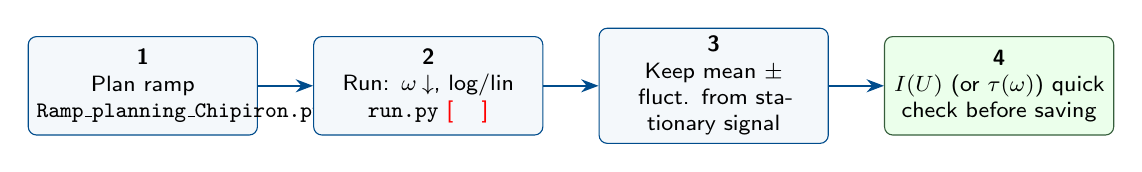
\begin{tikzpicture}[node distance=0.7cm]
\node[fstep,text width=2.7cm] (a) {\stepno{1}\\Plan ramp\\\code{Ramp\_planning\_Chipiron.py}};
\node[fstep,text width=2.7cm,right=of a] (b) {\stepno{2}\\Run: $\omega\!\downarrow$, log/lin\\\code{run.py} \fillme};
\node[fstep,text width=2.7cm,right=of b] (c) {\stepno{3}\\Keep mean $\pm$ fluct. from stationary signal};
\node[fok,text width=2.7cm,right=of c] (d) {\stepno{4}\\$I(U)$ (or $\tau(\omega)$) quick check before saving};
\draw[arr] (a)--(b); \draw[arr] (b)--(c); \draw[arr] (c)--(d);
\end{tikzpicture}
\end{figure}

\begin{table}[H]
\centering
\begin{tabularx}{\textwidth}{@{}l Y Y Y Y Y@{}}
\toprule
\textbf{Parameter} & \textbf{Range} & \textbf{N pts} & \textbf{Time / pt} & \textbf{Default field} & \textbf{Default lab} \\
\midrule
$\omega$ ramp (descending) & \fillme & \fillme & \fillme & \fillme & \fillme \\
Transient time & --- & --- & \fillme & \fillme & \fillme \\
Steady averaging window  & --- & --- & \fillme & \fillme & \fillme \\
Acquisition rate & \fillme & --- & --- & \fillme & \fillme \\
Repeats of full ramp  & --- & \fillme & \fillme & \fillme & \fillme \\
\bottomrule
\end{tabularx}
\caption{Ramp parameters.}
\end{table}

\begin{table}[H]
\centering
\begin{tabularx}{\textwidth}{@{}l Y@{}}
\toprule
\textbf{Record} & $U$, $\omega$, $I/\tau$, $t$ continuously over the whole ramp (full $I(t)$, $\tau(t)$ for each $\omega$) \\
\textbf{Look for} & steady value at each $\omega$; low-speed behaviour: yield-stress, intermittent motion/ arrest/strong fluctuations \\
\textbf{Output} & $\tau(\omega)$ with uncertainty / fluctuations at each point; repeatability; yield stress  \\
\textbf{Quick check} & live $\tau$ (or $I(U)$) vs.\ $\omega$: curve should increase and plateau (Fig.~\ref{fig:paul}) \\
\textbf{Later} & fit Herschel--Bulkley; dimensionless representation using inertia number $J$; compare results with plastic beads tests (PMMH) \\
\bottomrule
\end{tabularx}
\end{table}

\begin{figure}[H]
\centering
\safeimg[width=0.7\textwidth]{figures/pauletal2021.png}
\caption{Expected flow curves in frazil, from \cite{PaulEtAl2021}.}
\label{fig:paul}
\end{figure}


Foulques has tested asc/descending rotational speed ramps\textbf{from $1-70$ rpm}, using \textbf{10s} per point ( system  = plastic beads, Anton Paars rheometer).


\subsection{B --- Oscillatory: strain-amplitude sweep}\label{sec:osc}
\begin{figure}[H]
\centering
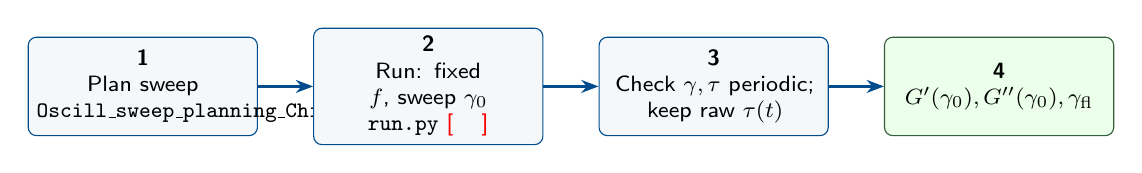
\begin{tikzpicture}[node distance=0.7cm]
\node[fstep,text width=2.7cm] (a) {\stepno{1}\\Plan sweep\\\code{Oscill\_sweep\_planning\_Chipiron.py}};
\node[fstep,text width=2.7cm,right=of a] (b) {\stepno{2}\\Run: fixed $f$, sweep $\gamma_0$\\\code{run.py} \fillme};
\node[fstep,text width=2.7cm,right=of b] (c) {\stepno{3}\\Check $\gamma,\tau$ periodic; keep raw $\tau(t)$};
\node[fok,text width=2.7cm,right=of c] (d) {\stepno{4}\\$G'(\gamma_0),G''(\gamma_0),\gamma_{\rm fl}$};
\draw[arr] (a)--(b); \draw[arr] (b)--(c); \draw[arr] (c)--(d);
\end{tikzpicture}
\end{figure}

\begin{table}[H]
\centering
\begin{tabularx}{\textwidth}{@{}l Y Y Y Y Y@{}}
\toprule
\textbf{Parameter} & \textbf{Range} & \textbf{N pts} & \textbf{Time / pt} & \textbf{Default field} & \textbf{Default lab} \\
\midrule
$\gamma_0$ sweep (log / lin) & \fillme & \fillme & \fillme & \fillme & \fillme \\
Cycles per point & --- & \fillme & --- & \fillme & \fillme \\
Forcing frequency $f$ (fixed) & \fillme & --- & --- & \fillme & \fillme \\
Settling time per point & --- & --- & \fillme & \fillme & \fillme \\
Sampling rate & \fillme & --- & --- & \fillme & \fillme \\
Repeats of full sweep  & --- & \fillme & \fillme & \fillme & \fillme \\
$f$ sweep in linear regime (lab, $G'(f),G''(f)$) & \fillme & \fillme & \fillme & --- & \fillme \\
\bottomrule
\end{tabularx}
\caption{Oscillatory parameters. }
\end{table}

\begin{table}[H]
\centering
\begin{tabularx}{\textwidth}{@{}l Y@{}}
\toprule
\textbf{Record} & imposed $\gamma(t)$ and $U(t)$, $f$, $\tau(t)$ or $I(t)$, number of cycles, $T$ \\
\textbf{Derive} & $G'$, $G''$, $\delta$, $\nu_{\rm eff}$; keep raw $\tau(t)$ and harmonic content if non-sinusoidal ( nonlinear / fluidised behaviour) \\
\textbf{Look for} & low-strain linear plateau, departure from linearity, change / crossing of $G'$ and $G''$, $\gamma_{\rm fl}$ \\
\textbf{Output} & $G'(\gamma_0)$, $G''(\gamma_0)$, $\delta$, raw $\tau(t)$, $\gamma_{\rm fl}$ where identifiable (lab: also $G',G''$ vs.\ $f$ ?) \\
\textbf{Quick check} & input and torque periodic and phase-resolved; qualitatively different regimes (Fig.~\ref{fig:Foulques_oscill}); repeatability \\
\bottomrule
\end{tabularx}
\end{table}

\begin{figure}[H]
\centering
\safeimg[width=0.5\linewidth]{figures/G'G''_labelled.png}
\caption{$G'(\gamma_0),\,G''(\gamma_0)$ in plastic beads (F.~Pillet).}
\label{fig:Foulques_oscill}
\end{figure}


Foulques has tested deformation sweeps \textbf{ $\gamma_0 = 10^{-4}-10^3 \%$} at $2\pi f = 0.5, ~ 5, ~10, ~15, ~20, ~25 $ rad/s, using \textbf{5s} per point, \textbf{60} points and \textbf{300s} intervals.  ( system  = plastic beads, Anton Paar rheometer). He also tried frequency sweeps: \textbf{$2\pi f = 10^{-1} - 10^{2}$ rad/s} at $\gamma_0 = 1\%$, and \textbf{$2\pi f = 10^{-2} - 10^{2}$ rad/s} at $\gamma_0 = 0.005\%$. One sweep takes about 5min for him. 


%=========================================================
\section{To-do and open questions}
%=========================================================
\begin{table}[H]
\centering
\begin{tabularx}{\textwidth}{@{}c Y@{}}
\toprule
$\square$ & \textbf{Item} \\
\midrule
$\square$ & Number of points per sweep, time per point, range, measurement-time estimate: field ramp, field oscillatory, lab ramp, lab oscillatory (tables in \S\ref{sec:protocols}) \\
$\square$ & Lab ramp: active measurement time (check Foulques' data) \\
$\square$ & Oscillatory (field and lab): time per amplitude sweep and per frequency sweep (check Foulques' notes) \\
$\square$ & Number of repeats: field ramp (3--4?), lab ramp (2--3?), amplitude sweeps (?) \\
$\square$ & Total time estimates per scenario; propose order of experiments with concrete times \\
$\square$ & Emphasis on repeatability vs.\ parameter change in field and in lab > do we agree on that?\\
$\square$ & Real command format for \code{run.py} (ramp and oscillatory); analysis and sample-characterisation scripts \\
$\square$ & Frazil state ($\phi,h_0$): measure just before or just after the run? \\
$\square$ & Lab oscillatory: do we do a  $f$ sweep in the linear regime ? \\
$\square$ & Calibration methods for $U\to\omega$ and $U\to\gamma$ (fill transit table) \\
$\square$ & Check order of steps!! eg: do we characterize samples before/after measurements? \\
$\square$ & Check Foulques' notes: how long is a typical experiment? Typical ranges?  \\
$\square$ & IMPORTANT: for fiels measurements, we'll probably be in cases where waves/wind introducs oscillatory components to measurements and change $\phi$,$h_0$ as we measure. So we can keep it simple and measure only using speed ramps at first order - this won't be that easy to understand.  \\
\bottomrule
\end{tabularx}
\end{table}

% bibliography
\addcontentsline{toc}{section}{Bibliography}
\nocite{DeLaRosaMaus2012,DeLaRosaMausKern2011}
\begin{thebibliography}{9}

\bibitem{DeLaRosaMaus2012}
S. De la Rosa and S. Maus,
``Laboratory study of frazil ice accumulation under wave conditions,''
\textit{The Cryosphere}, vol. 6, pp. 173--191, 2012.
\doi{10.5194/tc-6-173-2012}.

\bibitem{DeLaRosaMausKern2011}
S. De la Rosa, S. Maus, and S. Kern,
``Thermodynamic investigation of an evolving grease to pancake ice field,''
\textit{Annals of Glaciology}, vol. 52, no. 57, pp. 206--214, 2011.
\doi{10.3189/172756411795931787}.

\bibitem{MausDeLaRosa2012}
S. Maus and S. De La Rosa,
``Salinity and solid fraction of frazil and grease ice,''
\textit{Journal of Glaciology}, vol. 58, no. 208, 2012.
\doi{10.3189/2012JoG11J110}.

\bibitem{PaulEtAl2021}
F. Paul, T. Mielke, C. Schwarz, J. Schröder, T. Rampai, S. Skatulla,
R. R. Audh, E. Hepworth, M. Vichi, and D. C. Lupascu,
``Frazil Ice in the Antarctic Marginal Ice Zone,''
\textit{Journal of Marine Science and Engineering}, vol. 9, no. 6, p. 647, 2021.
\doi{10.3390/jmse9060647}.

\end{thebibliography}
\end{document}